% Options for packages loaded elsewhere
\PassOptionsToPackage{unicode}{hyperref}
\PassOptionsToPackage{hyphens}{url}
%
\documentclass[
  ignorenonframetext,
]{beamer}
\usepackage{pgfpages}
\setbeamertemplate{caption}[numbered]
\setbeamertemplate{caption label separator}{: }
\setbeamercolor{caption name}{fg=normal text.fg}
\beamertemplatenavigationsymbolsempty
% Prevent slide breaks in the middle of a paragraph
\widowpenalties 1 10000
\raggedbottom
\setbeamertemplate{part page}{
  \centering
  \begin{beamercolorbox}[sep=16pt,center]{part title}
    \usebeamerfont{part title}\insertpart\par
  \end{beamercolorbox}
}
\setbeamertemplate{section page}{
  \centering
  \begin{beamercolorbox}[sep=12pt,center]{part title}
    \usebeamerfont{section title}\insertsection\par
  \end{beamercolorbox}
}
\setbeamertemplate{subsection page}{
  \centering
  \begin{beamercolorbox}[sep=8pt,center]{part title}
    \usebeamerfont{subsection title}\insertsubsection\par
  \end{beamercolorbox}
}
\AtBeginPart{
  \frame{\partpage}
}
\AtBeginSection{
  \ifbibliography
  \else
    \frame{\sectionpage}
  \fi
}
\AtBeginSubsection{
  \frame{\subsectionpage}
}

\usepackage{amsmath,amssymb}
\usepackage{iftex}
\ifPDFTeX
  \usepackage[T1]{fontenc}
  \usepackage[utf8]{inputenc}
  \usepackage{textcomp} % provide euro and other symbols
\else % if luatex or xetex
  \usepackage{unicode-math}
  \defaultfontfeatures{Scale=MatchLowercase}
  \defaultfontfeatures[\rmfamily]{Ligatures=TeX,Scale=1}
\fi
\usepackage{lmodern}
\usetheme[]{Singapore}
\ifPDFTeX\else  
    % xetex/luatex font selection
\fi
% Use upquote if available, for straight quotes in verbatim environments
\IfFileExists{upquote.sty}{\usepackage{upquote}}{}
\IfFileExists{microtype.sty}{% use microtype if available
  \usepackage[]{microtype}
  \UseMicrotypeSet[protrusion]{basicmath} % disable protrusion for tt fonts
}{}
\makeatletter
\@ifundefined{KOMAClassName}{% if non-KOMA class
  \IfFileExists{parskip.sty}{%
    \usepackage{parskip}
  }{% else
    \setlength{\parindent}{0pt}
    \setlength{\parskip}{6pt plus 2pt minus 1pt}}
}{% if KOMA class
  \KOMAoptions{parskip=half}}
\makeatother
\usepackage{xcolor}
\newif\ifbibliography
\setlength{\emergencystretch}{3em} % prevent overfull lines
\setcounter{secnumdepth}{-\maxdimen} % remove section numbering


\providecommand{\tightlist}{%
  \setlength{\itemsep}{0pt}\setlength{\parskip}{0pt}}\usepackage{longtable,booktabs,array}
\usepackage{calc} % for calculating minipage widths
\usepackage{caption}
% Make caption package work with longtable
\makeatletter
\def\fnum@table{\tablename~\thetable}
\makeatother
\usepackage{graphicx}
\makeatletter
\def\maxwidth{\ifdim\Gin@nat@width>\linewidth\linewidth\else\Gin@nat@width\fi}
\def\maxheight{\ifdim\Gin@nat@height>\textheight\textheight\else\Gin@nat@height\fi}
\makeatother
% Scale images if necessary, so that they will not overflow the page
% margins by default, and it is still possible to overwrite the defaults
% using explicit options in \includegraphics[width, height, ...]{}
\setkeys{Gin}{width=\maxwidth,height=\maxheight,keepaspectratio}
% Set default figure placement to htbp
\makeatletter
\def\fps@figure{htbp}
\makeatother

\titlegraphic{\raisebox{-2cm}{
\includegraphics[width=2.5cm]{../20240214_SOT_ISES_Webinar/set-logo.jpg}}}
\makeatletter
\@ifpackageloaded{caption}{}{\usepackage{caption}}
\AtBeginDocument{%
\ifdefined\contentsname
  \renewcommand*\contentsname{Table of contents}
\else
  \newcommand\contentsname{Table of contents}
\fi
\ifdefined\listfigurename
  \renewcommand*\listfigurename{List of Figures}
\else
  \newcommand\listfigurename{List of Figures}
\fi
\ifdefined\listtablename
  \renewcommand*\listtablename{List of Tables}
\else
  \newcommand\listtablename{List of Tables}
\fi
\ifdefined\figurename
  \renewcommand*\figurename{Figure}
\else
  \newcommand\figurename{Figure}
\fi
\ifdefined\tablename
  \renewcommand*\tablename{Table}
\else
  \newcommand\tablename{Table}
\fi
}
\@ifpackageloaded{float}{}{\usepackage{float}}
\floatstyle{ruled}
\@ifundefined{c@chapter}{\newfloat{codelisting}{h}{lop}}{\newfloat{codelisting}{h}{lop}[chapter]}
\floatname{codelisting}{Listing}
\newcommand*\listoflistings{\listof{codelisting}{List of Listings}}
\makeatother
\makeatletter
\makeatother
\makeatletter
\@ifpackageloaded{caption}{}{\usepackage{caption}}
\@ifpackageloaded{subcaption}{}{\usepackage{subcaption}}
\makeatother
\ifLuaTeX
  \usepackage{selnolig}  % disable illegal ligatures
\fi
\usepackage{bookmark}

\IfFileExists{xurl.sty}{\usepackage{xurl}}{} % add URL line breaks if available
\urlstyle{same} % disable monospaced font for URLs
\hypersetup{
  pdftitle={Spatiotemporal Exposure and Toxicology \{SET\} Group},
  pdfauthor={Kyle P Messier, PhD},
  hidelinks,
  pdfcreator={LaTeX via pandoc}}

\title{Spatiotemporal Exposure and Toxicology \{SET\} Group}
\subtitle{2024 Tenure Track Advisory Committee Meeting}
\author{Kyle P Messier, PhD}
\date{}
\institute{National Institute of Environmental Health Sciences -
Division of Translational Toxicology - Predictive Toxicology Branch}

\begin{document}
\frame{\titlepage}

\renewcommand*\contentsname{Contents}
\begin{frame}[allowframebreaks]
  \frametitle{Contents}
  \tableofcontents[hideallsubsections]
\end{frame}
\section{Overview}\label{overview}

\begin{frame}{About Us}
\phantomsection\label{about-us}
\textbf{Spatiotemporal Exposures and Toxicology \{SET\} group}

\begin{itemize}
\tightlist
\item
  Geospatial Exposure Mapping: Spatiotemporal exposure mapping of
  environmental and climate variables (e.g.~chemical mixtures, social,
  behaviorial, environmental, and climate factors)
\item
  GeoTox: Otherwise known as \textbf{source to outcome continuum}
  modeling, GeoTox is the integration of geospatial exposures,
  toxicokinetic modeling, and non-animal toxicological data such as
  high-through \emph{in vitro} screen assays to develop
  mechanistically-informed risk maps of chemical mixtures
\item
  Software Development: Developing and promoting software and
  computational best-practices such as test driven development (TDD) and
  open-source code for the environmental health sciences
\end{itemize}
\end{frame}

\begin{frame}{About Us}
\phantomsection\label{about-us-1}
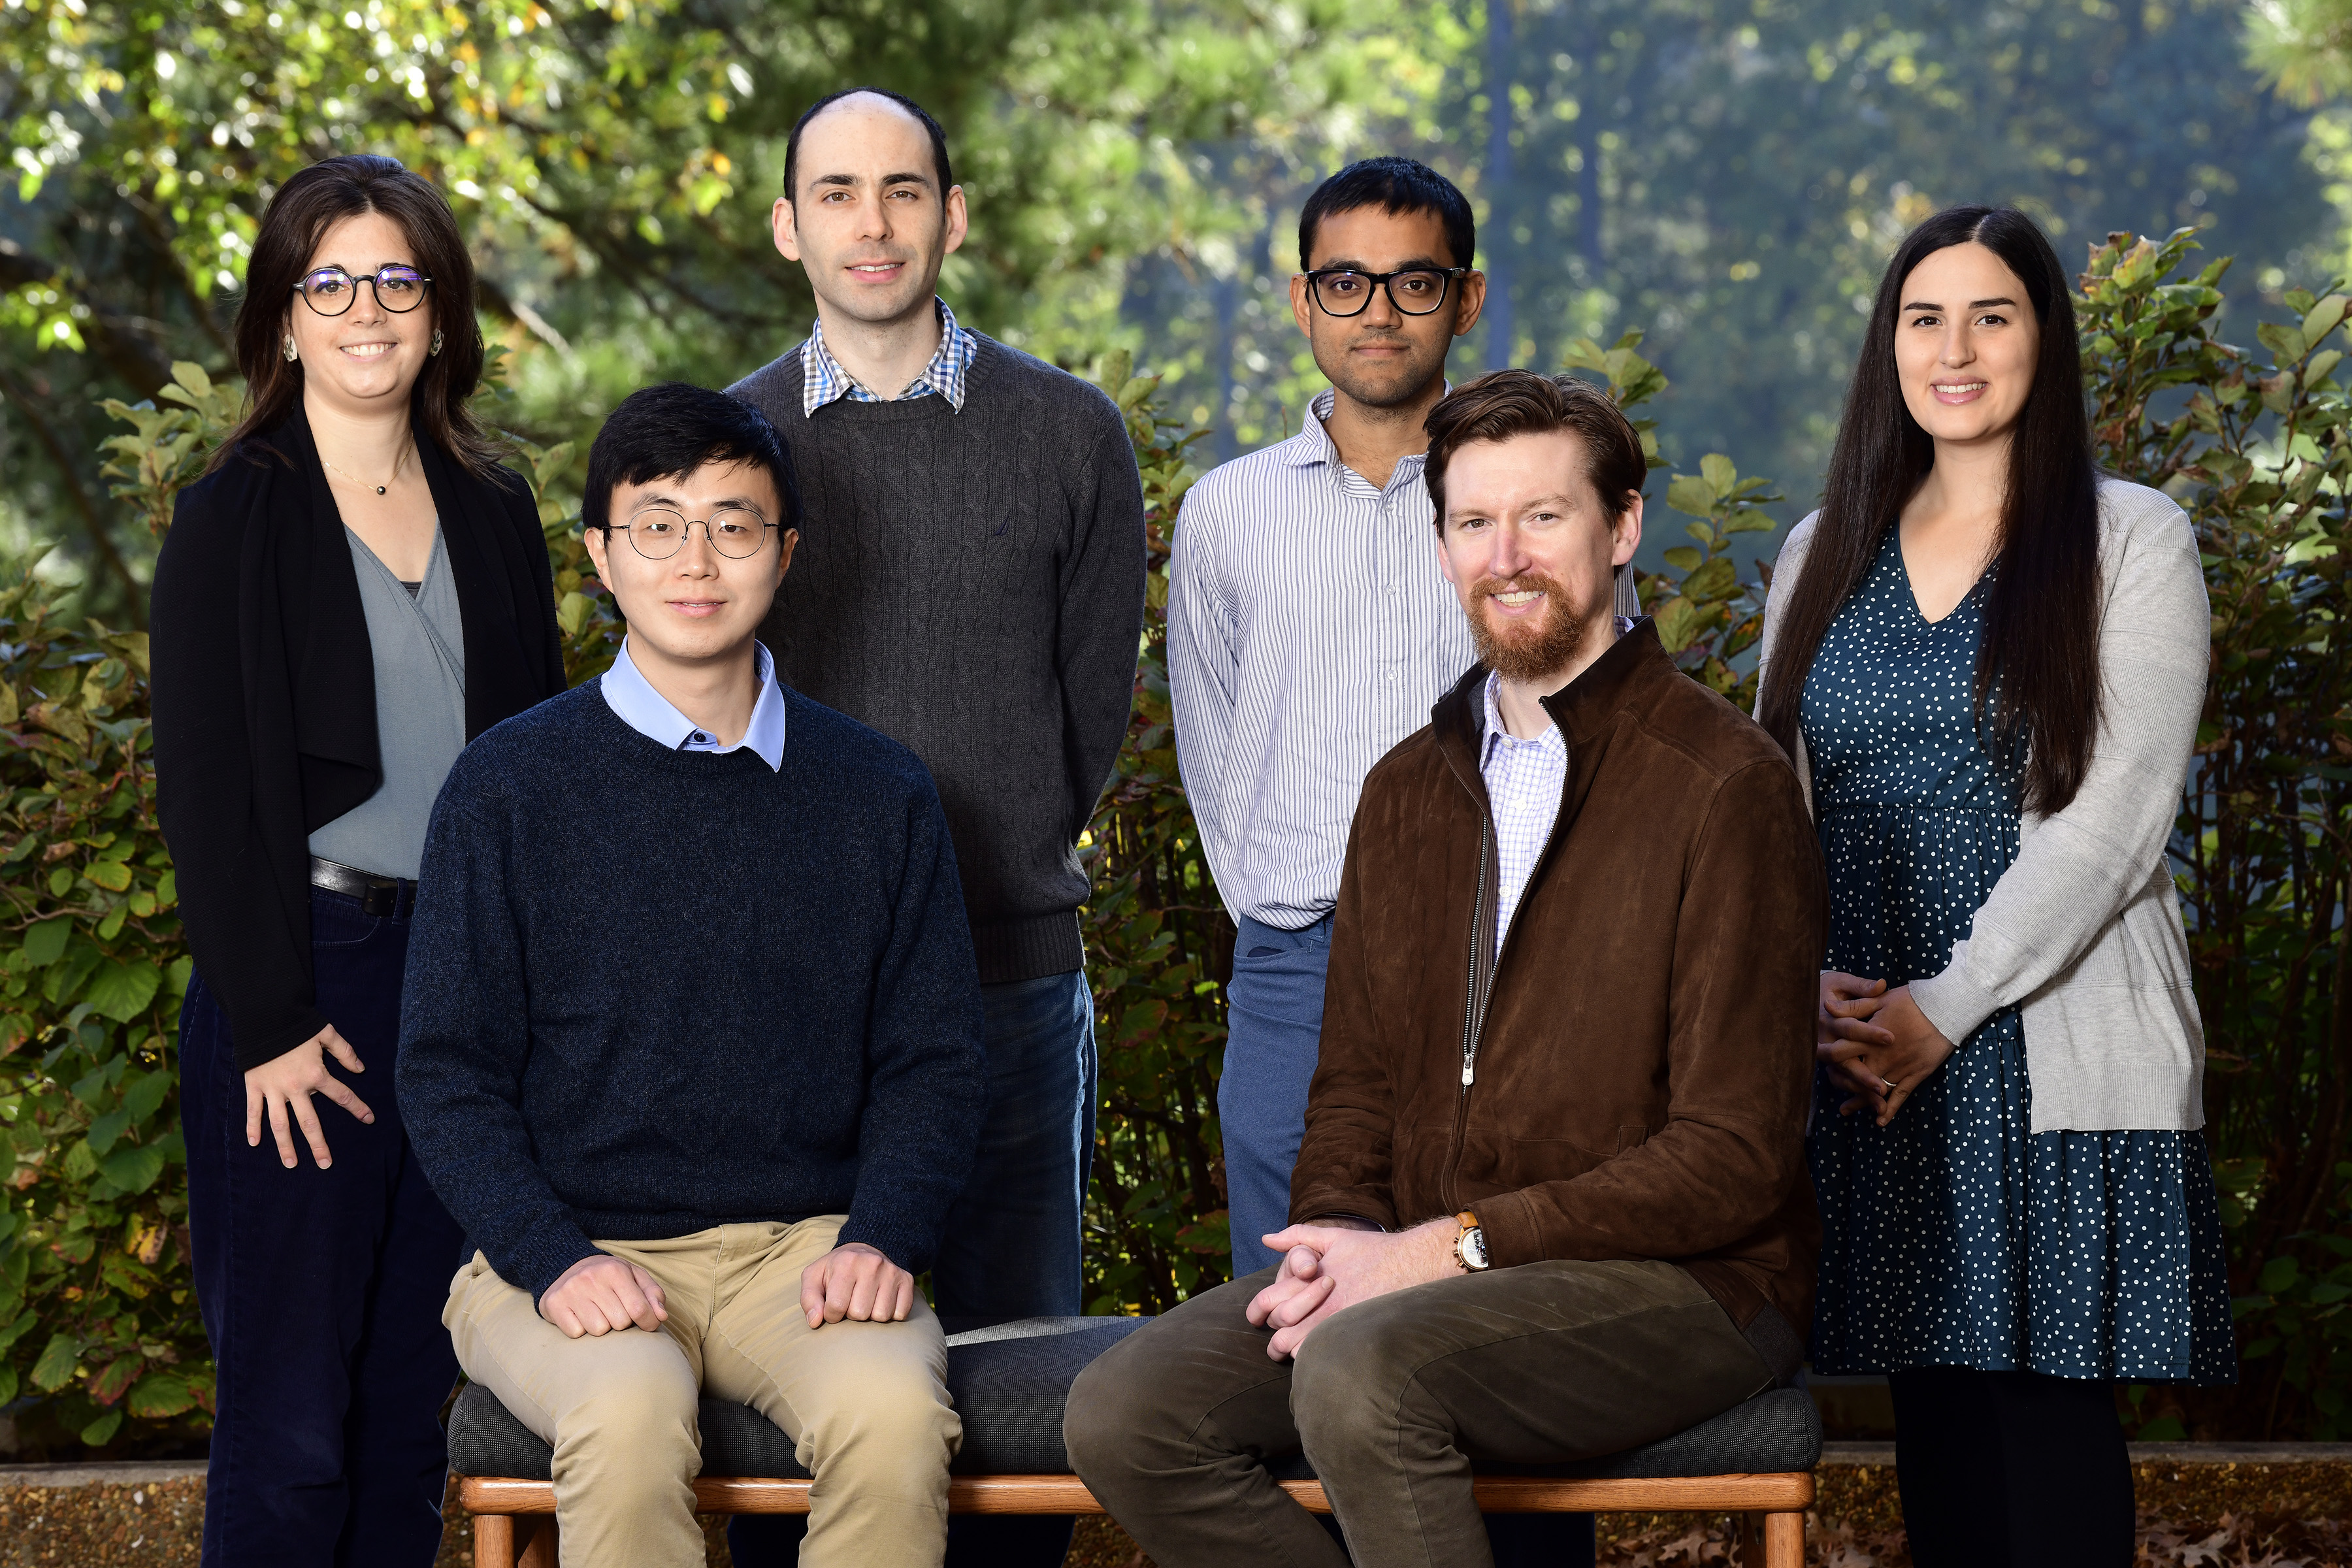
\includegraphics{../20240222_UNC_ESE_Guest_Lecture/SETgroup-Oct2023.jpg}
\end{frame}

\begin{frame}{CHORDS Project}
\phantomsection\label{chords-project}
\begin{itemize}
\tightlist
\item
  I am a co-lead on the CHORDS project with Aubrey Miller, Charles
  Schmitt, and Trisha Castranio.
\item
  David Reif, Alison Motsigner-Reif, David Fargo, among many others
  involved a regular contributors
\item
  The project represents a major NIEHS initiative for climate change and
  health research that I am involved in. It has come with additional
  monies for postdocs and data analysts in my group
\item
  It also comes with significant time commitments and responsibilities
\item
  A lot of the CHORDS work/deliverables are folded into my group's work
  and manuscripts
\end{itemize}
\end{frame}

\begin{frame}{Group Management}
\phantomsection\label{group-management}
\begin{itemize}
\tightlist
\item
  In late 2023/ early 2024, with help from the new CHORDS funding, my
  group was poised to expand from 2 postdocs to 5 postdocs and a data
  analyst.
\item
  I took 30 hours of project management courses to prepare
\item
  I adopted software best practices as both a technique to help manage
  the group and to improve the quality of our software products, as well
  as increase software as a product of our research group
\item
  Software best practices will help ensure that I have knowledge
  retention, reproducibility, and extensibility built into the core of
  my group

  \begin{itemize}
  \tightlist
  \item
    You'll see why this is important in the next few slides
  \end{itemize}
\end{itemize}
\end{frame}

\begin{frame}{Software and Computational Best Practices}
\phantomsection\label{software-and-computational-best-practices}
\begin{itemize}
\tightlist
\item
  Test Driven Development
\item
  Continuous Integration
\item
  Build Checks
\item
  Style/Linting
\item
  Workflows/Pipelines
\end{itemize}

\begin{center}
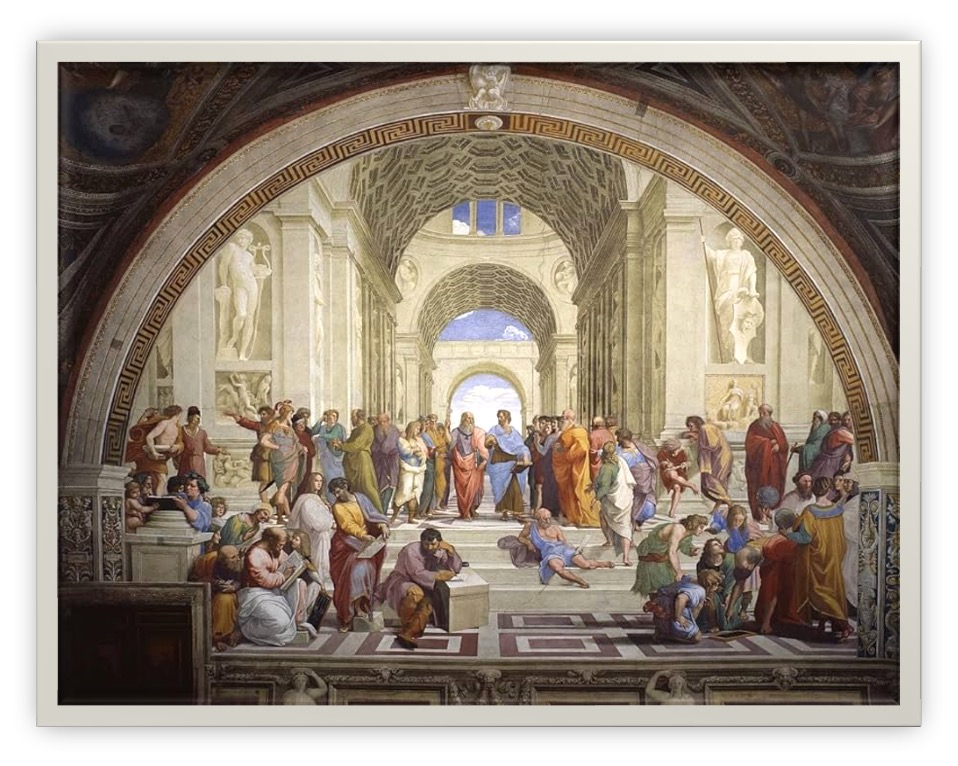
\includegraphics[width=0.4\textwidth,height=\textheight]{../../presentations/20240223_CEHD_Workshop/Raphael.jpg}
\end{center}
\end{frame}

\section{Group Personnel Updates}\label{group-personnel-updates}

\begin{frame}{Daniel Zilber}
\phantomsection\label{daniel-zilber}
\begin{itemize}
\tightlist
\item
  Postdoc with me \textasciitilde2.5 years
\item
  1 first/last author publication (Zilber and Messier, 2024)
\item
  1 first/second author publication (me 2nd, Matt Wheeler last) in major
  revisions
\item
  1 last/second (me last, Daniel 2nd) in press
\item
  Daniel is now a staff scientist with Shanshan Zhao as of July 7, 2024
  (BCBB)
\item
  Overall, Daniel has been an excellent postdoc and demonstrated how
  providing flexibility and intellectual freedom can lead to high-impact
  research
\end{itemize}
\end{frame}

\begin{frame}{Ranadeep Daw}
\phantomsection\label{ranadeep-daw}
\begin{itemize}
\tightlist
\item
  Postdoc with me 1 year
\item
  0 publications or products. 1 manuscript in progress, but not holding
  my breath for seeing it completed
\item
  Overall, disappointing, not meeting expectations, and negative
  attitude
\item
  Complained about data set being too large for the proposed
  methodology, then complained about it being too small
\item
  Nonetheless, a positive outcome as he accepted a position as a
  tenure-track assistant professor in Statistics at the University of
  West Florida
\end{itemize}
\end{frame}

\begin{frame}[fragile]{Insang Song}
\phantomsection\label{insang-song}
\begin{itemize}
\tightlist
\item
  Postdoc with me 1 year and as a contractor for 4 months before that
\item
  1st author publication in NIEHS internal review (\texttt{chopin}
  software manuscript).
\item
  1st author publication (\texttt{beethoven} group project) in
  preparation.
\item
  2nd author on \texttt{PrestoGP} manuscript in preparation
\item
  \textbf{Recent Big News} He has been offered and accepted a
  tenure-track assistant professor position at Seoul National University
  (Top Public University in Korea- Top 30-50 Worldwide). It is a great
  opportunity for him for a highly competitive position. A bit
  bittersweet for me because he has been an amazing postdoc and
  extremely productive.

  \begin{itemize}
  \tightlist
  \item
    Start date is surprisingly soon, Sept 1 2024.
  \end{itemize}
\end{itemize}
\end{frame}

\begin{frame}{Eva Marques}
\phantomsection\label{eva-marques}
\begin{itemize}
\tightlist
\item
  Postdoc with me 1 year
\item
  Excellent group member and attitude
\item
  Project on high-resolution heat exposure mapping is going well

  \begin{itemize}
  \tightlist
  \item
    2 first author publications in progress. 1 first author publication
    in 2025 is realistic.
  \end{itemize}
\end{itemize}
\end{frame}

\begin{frame}{Mariana Alifa Kassien}
\phantomsection\label{mariana-alifa-kassien}
\begin{itemize}
\tightlist
\item
  Postdoc with me 1 year
\item
  Excellent group member and positive attiude
\item
  Project goal is to develop a geospatial of 100+ VOCs in air.

  \begin{itemize}
  \tightlist
  \item
    The methodology has changed from a physics-informed neural network
    to something more tractable that builds upon our previous spatial
    models and pipeline developments.
  \item
    Additionally, we hope to integrate this into the \textbf{GeoTox}
    framework towards a geospatial mixtures risk assessment.
  \end{itemize}
\item
  Spends 10-20\% of her time working with the CHORDS knowledge
  dissemination team and has some interest science communication and
  outreach.
\item
  Was on maternity leave from Mar - May 2024.
\end{itemize}
\end{frame}

\begin{frame}[fragile]{Mitchell Manware}
\phantomsection\label{mitchell-manware}
\begin{itemize}
\tightlist
\item
  With me 1 year as a fully-remote data analyst supported by the CHORDS
  project.
\item
  Has been a great team member contributing to \texttt{amadeus} and
  \texttt{beethoven} software as well as leading the first-author for
  the \texttt{amadeus} manuscript (currently under internal NIEHS
  review).
\item
  He is interested in doing a PhD with the goal of learning and
  developing ML/AI models for environmental exposure and risk
  assessment, but has a likely geographical constraint of New England.
  Will discuss the possibility of supporting a PhD at UNC ESE.
\end{itemize}
\end{frame}

\begin{frame}{Postbac Outcomes}
\phantomsection\label{postbac-outcomes}
\begin{itemize}
\item
  \textbf{Taylor Potter}, BS, IRTA Postbac 2020-2022, now in MD program
  at Meherry Medical College
\item
  \textbf{Melissa Lowe}, BS, MS, IRTA Postbac 2020-2022, 1st author
  publication, Biostatistician at Duke Cancer Center, Recently resigned
  to purse a JD and focus on environmental justice, I wrote her a
  recomomendation letter for law school.
\end{itemize}
\end{frame}

\begin{frame}{Postdoc Outcomes}
\phantomsection\label{postdoc-outcomes}
\begin{itemize}
\item
  \textbf{Dr.~Kristin Eccles} - Research Scientist, Computational
  Toxicology Research group, Exposure and Biomonitoring Division, Health
  Canada
\item
  \textbf{Dr.~Ranadeep Daw} - Tenure Track Assistant Professor,
  Department of Mathematics and Statistics, University of West Florida
\item
  \textbf{Dr.~Daniel Zilber} - Staff Scientist, BCBB, NIEHS
\item
  \textbf{Dr.~Insang Song} - Tenure Track Assistant Professor, Seoul
  National University
\end{itemize}
\end{frame}

\begin{frame}{Summer Intern Outcomes}
\phantomsection\label{summer-intern-outcomes}
\begin{itemize}
\item
  \textbf{Alvin Sheng}, PhD candidate, SIP 2021, NCSU Department of
  Statistics (Advisor: Brian Reich), Project manuscript is now in press
  in American Journal of Epidemiology, Included as 3rd chapter in
  dissertation.
\item
  \textbf{Jennifer Kampe}, PhD candidate, SIP 2024, Duke Department of
  Statistics (Advisor: David Dunson), Project is on the development of a
  Bayesian latent variable model for chemical mixture prediction. She is
  hoping it can be incorporated into her dissertation.
\end{itemize}
\end{frame}

\section{Project Updates}\label{project-updates}

\begin{frame}[fragile]{PrestoGP}
\phantomsection\label{prestogp}
\begin{itemize}
\item
  \texttt{PrestoGP} and the application on US-wide groundwater
  pesticides is proceeding with steady progress. The publication is in
  preparation, but we are unlikely to get it done in 2024. Nonetheless,
  I am still excited at this development and the potential for a
  high-impact publication in late 2024 or 2025.
\item
  Jump over to \texttt{PrestoGP} GitHub repo and website:
  https://niehs.github.io/PrestoGP/
\end{itemize}
\end{frame}

\begin{frame}{\texttt{beethoven} SET Group Project}
\phantomsection\label{beethoven-set-group-project}
\begin{itemize}
\tightlist
\item
  Goal: Develop an air pollution model for the last 5 years that is
  updated bi-annually
\item
  Entire SET group, Cavin Ward-Caviness, Lara Clark, Anisha Singh
\item
  Test-Driven Development
\item
  GitHub with strict rules
\item
  Targets make-like pipeline
\item
  Fine spatial and temporal resolution
\item
  Post-processing for aggregated spatial and temporal resolutions
\end{itemize}
\end{frame}

\begin{frame}{\texttt{beethoven} pipeline overview}
\phantomsection\label{beethoven-pipeline-overview}
\includegraphics{IS-slide-export/Slide2.jpeg}
\end{frame}

\begin{frame}{\texttt{beethoven} pipeline implementation}
\phantomsection\label{beethoven-pipeline-implementation}
\includegraphics{IS-slide-export/Slide3.jpeg}
\end{frame}

\begin{frame}{\texttt{beethoven} targets pipeline}
\phantomsection\label{beethoven-targets-pipeline}
\includegraphics{IS-slide-export/Slide4.jpeg}
\end{frame}

\begin{frame}{\texttt{GeoTox} package development}
\phantomsection\label{geotox-package-development}
\begin{itemize}
\tightlist
\item
  Working with David Reif and Skylar Marvel to develop the
  \textbf{GeoTox} framework into an open-source, extensible, R-package.
\item
  Manuscript in preparation for special issue in \textbf{Human
  Genomics}. Expect to have draft in the next month or two.
\item
  Incorporating multi-assay chemical risk characterization
\end{itemize}
\end{frame}

\begin{frame}{\texttt{GeoTox} package development}
\phantomsection\label{geotox-package-development-1}
\includegraphics[width=\textwidth,height=0.8\textheight]{GeoTox.png}
\end{frame}

\section{Summary and Looking Forward}\label{summary-and-looking-forward}

\begin{frame}{SET Software}
\phantomsection\label{set-software}
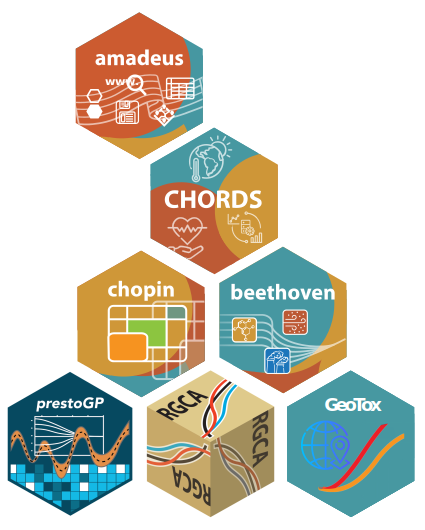
\includegraphics[width=0.6\textwidth,height=\textheight]{SET-software-chorus.png}
\end{frame}

\begin{frame}[fragile]{2024}
\phantomsection\label{section}
\begin{itemize}
\tightlist
\item
  2023/2024 was spent doing lots of logistical work and project
  management
\item
  On-boarding of a large group and setting up projects
\item
  TDD and software development practices has helped ensure that we are
  building robust and reproducible software and that I can trust what
  are large team is doing without having to micromanage
\item
  Some publications such as \texttt{PrestoGP} were not finished, but
  steady progress is being made and I am optimistic about the potential
  for high-impact publications in 2025
\end{itemize}
\end{frame}

\begin{frame}[fragile]{2025}
\phantomsection\label{section-1}
\begin{itemize}
\tightlist
\item
  Analytical pipelines and tools have been developed, which should make
  my life easier and more productive
\item
  I am excited about the potential for high-impact publications in 2025
\item
  BSC preparation is starting

  \begin{itemize}
  \tightlist
  \item
    The two \texttt{GeoTox} manuscript (POY and package development)
    will considered as publications to highlight
  \item
    \texttt{PrestoGP} and \texttt{beethoven} will be good to highlight
    as current and future progress
  \item
    Good trainee outcomes will be highlighted
  \item
    Climate and health research (AJE pub, CHORDS)
  \item
    Software development and open science (GeoTox, PrestoGP, beethoven)
  \end{itemize}
\end{itemize}
\end{frame}

\begin{frame}{Hiring}
\phantomsection\label{hiring}
\begin{itemize}
\tightlist
\item
  I have base funding for 2 postdocs (replacing Daniel Zilber and
  Ranadeep Daw)
\item
  I have options through CHORDS to hire data analysts and utilize SOARS
  (Replacing Insang Song)
\item
  I have options through PTB, perhaps combined with SET group CAN, to
  support a PhD student
\end{itemize}
\end{frame}



\end{document}
